\documentclass{sig-alternate}
\usepackage{multirow}
\usepackage[usenames, dvipsnames]{color}
\usepackage{colortbl}

\usepackage{balance}

\usepackage{times}
\usepackage{tabularx}
\usepackage{subcaption}
\usepackage{picture}
\usepackage{wrapfig}
\usepackage{algorithm}
\usepackage{graphicx}
\usepackage{algorithmicx}
\usepackage{algpseudocode}
\renewcommand{\algorithmicrequire}{\textbf{Input:}}
\renewcommand{\algorithmicensure}{\textbf{Output:}} 
\newcommand{\lucas}[1]{\textcolor{red}{LUCAS: #1}} 
\newcommand{\tim}[1]{\textcolor{Red}{TIM: #1}}
\newcommand{\bill}[1]{\textcolor{blue}{BILL: #1}} 
\newcommand{\carter}[1]{\textcolor{cyan}{CARTER: #1}} 
\newcommand{\sei}[1]{\textcolor{RedViolet}{BILL/FORREST: #1}} 
\newcommand{\todo}[1]{\textcolor{Maroon}{TODO: #1}} 
%\newenvironment{changed}{\par}{\par}

%timm tricks
\newcommand{\bi}{\begin{itemize}}%[leftmargin=0.4cm]}
\newcommand{\ei}{\end{itemize}}
\newcommand{\be}{\begin{enumerate}}
\newcommand{\ee}{\end{enumerate}}
\newcommand{\tion}[1]{\S\ref{sect:#1}}
\newcommand{\fig}[1]{Figure~\ref{fig:#1}}
\newcommand{\eq}[1]{Equation~\ref{eq:#1}}
 

\usepackage[shortlabels]{enumitem} 
%\usepackage{times}

\usepackage{cite}
\newcommand{\subparagraph}{}
\usepackage{url}
\def\baselinestretch{1}


%\setlist{nosep}

\usepackage{colortbl}
 %\usepackage[font={small}]{caption, subfig}
%\setlength{\abovecaptionskip}{1ex}
 %\setlength{\belowcaptionskip}{1ex}
% \setlength{\floatsep}{1ex}
% \setlength{\textfloatsep}{1ex}
%\usepackage[compact,small]{titlesec}
\DeclareMathSizes{7}{7}{7}{7} 
\pagenumbering{arabic}
%\setlength{\columnsep}{7mm}

\begin{document}

\conferenceinfo{ICSE}{'16 Austin, Texas}
\title{Live and Let Die? (Delayed Issues   not  Harder to Resolve)}
\numberofauthors{3}
\author{
%\alignauthor 
Tim Menzies \\
       \affaddr{Computer Science}\\
       \affaddr{NC State University, USA}\\
       \email{tim.menzies@gmail.com}
\and%alignauthor 
William Nichols, Forest Shull \\
        \affaddr{Software Engineering Institute}\\
        \affaddr{Carnegie Mellon U, USA}\\
        \email{\{wrn,fjshull\}@sei.cmu.edu} 
\and %\alignauthor 
Lucas Layman \\
       \affaddr{Fraunhofer CESE} \\
       \affaddr{College Park, USA}\\ 
       \email{llayman@fc-md.umd.edu}
} 
\maketitle
\begin{abstract}
Many  practitioners and academics
believe in a delayed issue effect (DIE); i.e.
 as issues linger longer in a system,
 they become exponentially harder to resolve.
This belief
is often  used to justify 
major investments in  new development
processes that promise to retire more issues, sooner.

This paper checks for the delayed issue effect in
171 software projects from around the world (2006 to 2014).
To the best of our knowledge,  this is the largest study
yet published on this effect.
What was observed was the  exact
opposite of the  delayed issue effect. Specifically:
the  time  to resolve 
issues  in one phase  was rarely more than when  issues
were resolved at a later phase. 

This  result begs the question: how many other long-held
beliefs in software engineering are
unsupported by current data? 
\end{abstract}

%XXXwhat it this is due to TSP- 
% A category with the (minimum) three required fields
\vspace{1mm}
\noindent
{\bf Categories/Subject Descriptors:} 
D.2.8 [Software Engineering]: Process metrics.

 

\vspace{1mm}
\noindent
{\bf Keywords:} software economics, phase delay, cost to fix.
 

\section{Introduction}
In 2013-2014, 
eleven  million programmers~\cite{pettey14} and
half a trillion dollars~\cite{avram14} were spent on information technology.
Such a large and growing effort should be managed and optimized via  well-researched conclusions.  

It is standard practice
in other fields such as medicine,
to continually revisit old conclusions~\cite{prasad13}.
Accordingly, this paper revisits
the widely-held belief of a {\em delayed issue effect} (hereafter, DIE).
Later in this paper, we offer a precise definition for this effect.
For the moment, we describe it as follows:
it is far easier to resolve issues earlier than later in the lifecycle.
 \fig{b81} shows an example of the delayed issue effect (relating
 the relative cost of fixing requirements issues at different phases of a project).
 
 Basili \& Boehm comment that since the 1980s,  this effect
 \begin{quote}
``...has been a major driver in focusing
industrial software practice on thorough
requirements analysis and design,
on early verification and validation, and
on up-front prototyping and simulation
to avoid costly downstream fixes''~\cite{boehm01}.
\end{quote}
 \begin{figure}[!b]  
\begin{center}
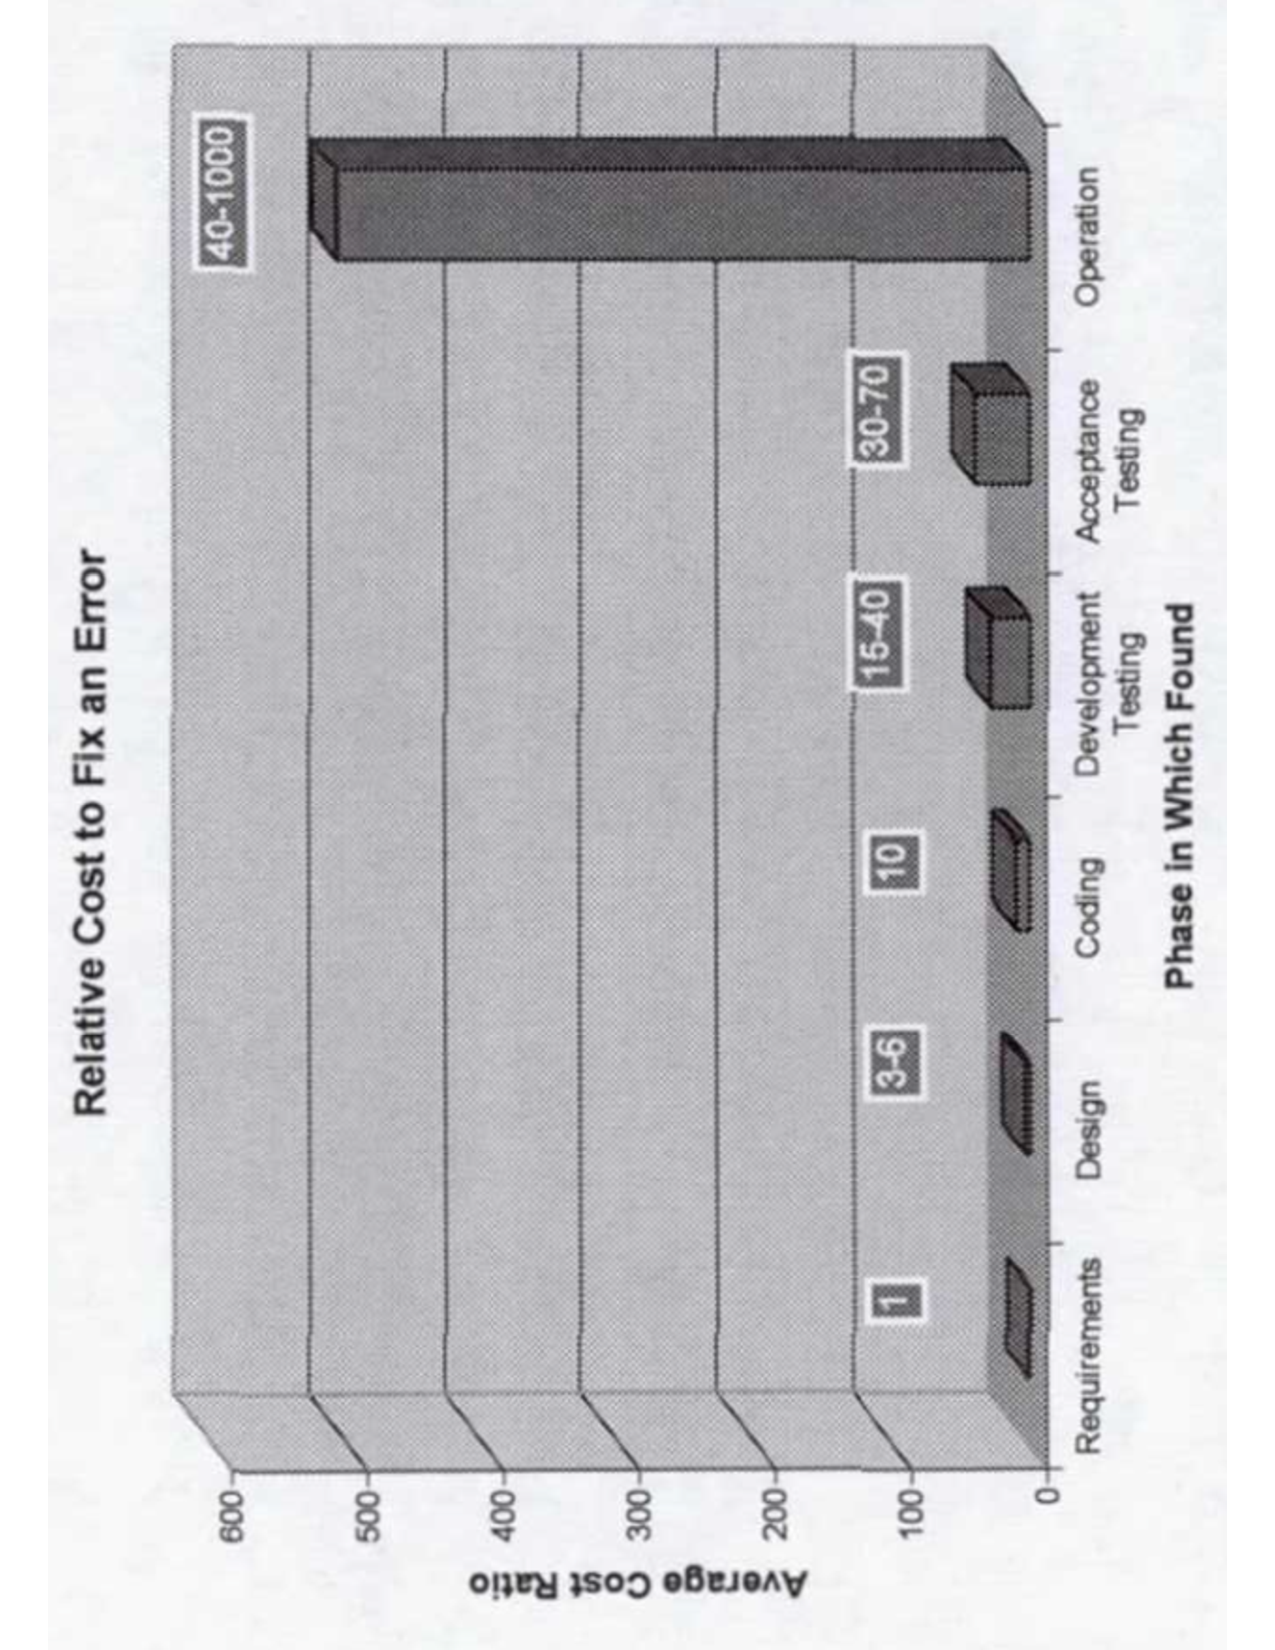
\includegraphics[angle=270,width=3in]{img/b81.pdf}
 \end{center}
 \caption{An example DIE effect. From Boehm'81~\cite{Boehm81}. }\label{fig:b81}
 \end{figure}
Other prominent authors have commented on its perceived usefulness as a rule of thumb for software engineers.  McConnell mentions it as a "common observation" in the field and  summarizes the intuitive argument for why it should be so: 
\begin{quote}
''A small mistake in upstream work can affect large amounts of downstream work. A change to a single sentence in a requirements specification can imply changes in hundreds of lines of code spread across numerous classes or modules, dozens of test cases, and numerous pages of end-user documentation''~\cite{mcconnell01}. 
\end{quote}
Glass also endorses this effect, asserting that``requirements errors are the most expensive to fix when found during production but the cheapest to fix early in development'' is ``really just common sense''~\cite{glass02}.  Other researchers
are just as adamant in asserting that that the delayed issue effect is a proven
fact.
For example, what we call the delayed issued effect was listed as number one by Boehm and Basili in their "Top 10 list" of ``objective and quantitative data, relationships,
and predictive models that help
software developers avoid predictable pitfalls
and improve their ability to predict
and control efficient software projects''~\cite{boehm01}.
 

% \begin{figure}[!t]
% \scriptsize
% \begin{center}
% \begin{tabular}{l@{~}|l@{~}|r@{~}r@{~}|r@{~}l}
%           &        & \multicolumn{2}{c|}{Time to}  &\\
%           &        & \multicolumn{2}{c|}{resolve} &\\
% Injection & Removal& initial & now & \multicolumn{2}{l}{Scale up w.r.t initial} \\\hline
% Phase $i$&Phase $i$ & 1 & 1 & 1 & **\\
% Phase $i$ &Phase $i+1$ & 1 & 2& 2 & **** \\
% Phase $i$ &Phase $i+2$ & 1 & 4& 4 &******** \\
% Phase $i$ &Phase $i+3$ & 1 & 8 & 8 & ****************  
%   \end{tabular}\end{center}
%  \caption{Projects data consistent with
%  the phase delay effect of \fig{curve1}.}\label{fig:curve1a}
% \end{figure}

% \begin{figure}[!t]
% \scriptsize
% \begin{center}
% \begin{tabular}{l@{~}|l@{~}|r@{~}r@{~}|r@{~}l}
%           &        & \multicolumn{2}{c|}{Time to}  &\\
%           &        & \multicolumn{2}{c|}{resolve} &\\
% Injection & Removal& initial & now & \multicolumn{2}{l}{Scale up w.r.t initial} \\\hline
% Phase $i$&Phase $i$ & 1 & 1 & 1 & ** \\
% Phase $i$ &Phase $i+1$ & 1 & 2& 2 & **** \\
% Phase $i$ &Phase $i+2$ & 1 & 2& 2 & **** \\
% Phase $i$ &Phase $i+3$ & 1 & 2 & 2 & **** \\
%  Phase $i$  &Phase $i+4$ &1 & 2& 2 &**** 
%   \end{tabular}\end{center}
%  \caption{Projects data consistent with
%  the phase delay effect of \fig{curve2}.}\label{fig:curve2a}
% \end{figure}
This paper calls into question all the above claims about the delayed
issue effect. We suggest that the delayed issue effect might have been an dominant
effect decades ago,  but {\em not}  for $21^{\mathit{st}}$
software development. 
 The delayed issue effect was first reported in 1981 in a era of punch card programming
and non-interactive environments~\cite{Boehm81}. In the 21$^\mathit{st}$ century, we  program in 
interactive environments with higher-level languages and better source code control
tools. Such tools allow for the faster refactoring of existing
code-- in which case, 
managing the changes required to fix (say) an incorrect requirements assumption
is far less    onerous    than before.

Also, we note that our development practices have changed in ways that could   mitigate the delayed issued effect.  Previously,
software was large monolithic systems that were write once and maintain
forever. Today, there are more architectures that
support  extensive and faster changes to software. 
For example, 
Microsoft is adjusting its development practices towards a continuous
release paradigm. Theisen et al. reports their experiences where Microsoft architects
continually adjust  their modules in response to security issues~\cite{theisen15}.
Also, upgrades to their Windows operating system is moving from service patches (which occur rarely) to continuous deployment (so there will be no Windows 11- just a stream of continuous updates to what is currently called Windows 10~\cite{bright15}).

For another example, consider the MEAN stack preferred for web development by
the continuous deployment community. Older architectures for web development
often used some variant of LAMP (Linux + Appache + Mysql + PHP) that was an intricate
combination of tools written in different languages. MEAN stacks, on the other hand,
use Javascript throughout-- which makes large scale reorganizations faster to complete~\cite{wayner15}. 

Inspired by the success of agile approaches, other  development organizations are similarly reorganizing their work-- witness the US Department of Defense's 2010 mandate
that all new software acquisitions must adopt agile methods~\cite{kim13}. 
This change in DoD policy arises from a separation of baseline architecture
(e.g. the design of an 
aircraft carrier) and the development of applications within that architecture.
For the baseline architecture, bad decisions
made  early in the life cycle may be too expensive to change.
But at least at the DoD, the majority of software development occurs within
the framework of some larger architecture (e.g. an aircraft carrier).
These smaller projects can certainly lever the agile advantage, while 
using fast refactoring tools that mitigate against  the delayed issue effect.

The above argument is an anecdotal evidence that  the delayed issue effect might no longer exist. But anecdotes are not really rigorous
evidence. Accordingly,  this article explores the currency of the delayed issue effect.
After some initial definitions, we discuss the
value of checking old ideas. Next, a survey of industrial practitioners and researchers to document a widespread belief that delayed issues have a negative impact on projects.  After that, we  analyze 171 software  projects developed in the period 2006 to 2014 to find  {\em no evidence} of the delayed issue effect:
\bi
\item
To ensure reproducibility,
all the data  used in this study is available in the PROMISE
repository at openscience.us/repo. 
\item
To the best of our knowledge,
this the largest study devoted the delayed issue effect yet conducted.
\ei
Finally, we discuss the validity and implications of our results.
 
\section{Definitions \& Hypotheses}
This paper uses the following definitions:
\bi
\item
The {\em delayed issue effect}:   it is {\em exponentially}  more {\em difficult} to resolve  issues in a software project, the {\em longer} they remain.
\item
 {\em Longer} time is defined as per  Boehm'81~\cite{Boehm81}; i.e. the gap between the   phases where   issues are introduced and resolved.
\item
A measure collected in phase ${1,.,i,..j}$ is 
{\em exponential} when  that
   measure at phase $j$   
   is larger than the sum of that measure in 
earlier phases $1 \le i < j$. 
\item
Issues are more {\em difficult}  
when their resolution takes more time or costs more  (e.g. needs expensive
debugging tools or the skills of expensive developers).
\ei
Note that we use  the  term ``delayed issue effect'' as generalization of the
more specific rule  ``requirements errors are hardest to fix''.
This generalization is valid since the rationale for the rule about requirements
is usually done as per McConnell~\cite{mcconnell01}; i.e. small upstream mistakes very
early in the system can cascade into huge problems later in the lifecycle.
That said, we prefer our more general term ``delayed issue effect'' since not
only might requirements errors cascade, so too might analysis errors, design errors, etc.



This paper defends the  following claims. Note that we call them
``claims'' not ``hypotheses'' since the later require defense via some statistical
significance test. On the other hand, our claims will be supported via a variety
of arguments, presented later in this paper.

{\bf  Claim1: ``DIE'' is a  widely-held belief.}
Using a literature review, we can confirm that there are numerous historical papers (dating back decades)
that endorse DIE. Also, using a survey conducted from this paper, we find  that 
  DIE  appears up as the
single most strongly-held beliefs amongst commercial software engineers.

{\bf  Claim2: ``DIE'' is a poorly documented.}
 As discussed in our literature review,  many of the papers reporting the DIE
effect are either (1)~quite old (papers dating from last century);
(2)~that just quote prior papers without presenting   new data; 
(3)~or cite data sources that can no longer be
confirmed. 

{\bf Claim3: Delayed Issues not Harder to Resolve.}
 In our sample of 
 171 software  projects developed, we will show
{\em no evidence}  that, during development, delayed issues were exponentially harder to resolve the longer they were left
 in the software. 
 


 


% the SE community needs to stop
% justifying changes to SE
% practices via the phase delay effect. Secondly,   myths like phase delay should not have lasted decades
% in the literature without  critical reassessment.  As a community, we need to reflect more on our
% research practices and on how (and when) we reflect and revisit the prominent hypotheses of our field.
  



\section{ But Why Reassess Old Truisms?}

Before going any further,  we digress to discuss the merits of revisiting
old conclusions in software engineering.


Beliefs in general
principles of software
engineering are common to both research and practice. Professional societies assume such generalities exist when they offer
 lists of supposedly general ``best practices'' such as
the IEEE 1012 standard for software verification~\cite{1012}. 
 Endres \& Rombach offer dozens of lessons of software engineering~\cite{endres03}.
 Many other 
widely-cited researchers  do the same; e.g.
Glass~\cite{glass02}; Jones~\cite{jones07}; Boehm~\cite{boehm00b}.
Budgen \& Kitchenham seek to reorganize SE research using
general
conclusions drawn from a larger number of studies~\cite{kitch04,budgen09}.

That said, there are many empirical  findings that 
raise doubts that   general laws of SE even exist:
\be
\item
Turhan~\cite{me12d} lists 28 studies with contradictory conclusions
on the relation of OO measures to defects.  Those results
 directly  contradict some of the laws listed by 
Endres \& Rombach~\cite{endres03}.
\item
Ray et al.~\cite{ray2014lang} tested if   strongly typed languages
predict for better code quality. In  728 projects,
they found  only a modest benefit in strong typing
(and caution that that effect may actually be due to other  conflating factors).
\item
Fenton \& Neil~\cite{fenton00,fenton00b}   critique the truism that
``pre-release fault rates for software
are a predictor for post-release failures'' (as claimed by~\cite{dunsmore88},
amongst others). For the systems described in~\cite{fenton97}, they
show that software modules that were highly fault-prone
prior to release revealed very few faults after release.
\item
Meyer claims that   object-oriented (OO) encapsulation will
reduce error rates in software~\cite{Meyer1988}.  Yet empirical results suggest
that debugging an OO program is many times harder and
longer than debugging a standard procedural program~\cite{hatton98}.
\item
A truism of visual programming is that ``visual
representations are inherently superior to mere textual representations''. A review by Menzies suggests that the available
evidence for this claim is hardly conclusive~\cite{me00v}. 
\item
Numerous recent {\em local learning} results compare single models
learned from all available data to multiple models learned from clusters within the data~\cite{betten14,yang11,yang13,minku13,me12d,me11m,betta12,posnett11}.
A repeated result in those studies in that the local models generated the better effort
and defect predictions (better median results,
lower variance in the predictions).
\ee
% \item 
% Other work studies  found dozens of single
% models that performed worse that {\em committees of models}, all with % different opinions,
% that contribute to an {\em ensemble} prediction of software 
% development effort~\cite{kocaguneli2012value,azhar13}.
To be fair, 
SE is  not the only
field where practitioners hang on to persistent beliefs, even if the evidence
for those beliefs is not strong.
The medical profession applies  many practices based on studies
that have been disproved. For example,
a  recent article
in the Mayo Clinic Proceedings~\cite{prasad13} found  
146 medical practices based on studies 
in year $i$, but which were  reversed by subsequent trials within years $i+10$.
Even when the evidence for or against a treatment or intervention is clear, medical providers and patients may not accept it~\cite{aschwanden10}.
Aschwanden warns that ``congitive biases''  such as  confirmation bias (the tendency to look for evidence that supports what you already know and to ignore the rest)  influence how we process information~\cite{aschwanden15}.

The cognitive issues that complicate medicine are also found in software engineering.
According to Passos et al.~\cite{passos11}, commercial developers
are all too willing to believe in general
truisms.
They  warn that developers
usually assume that the truisms they learn from a few past
projects are general to 
all their future projects. They comment ``past experiences were taken into account without 
much consideration for their context~\cite{passos11}.  
The results of J{\o}rgensen \& Gruschke~\cite{jorgensen09} concur with Passos et al. They report that 
  supposed software engineering    ``experts'' rarely use lessons
  from past projects to improve their future reasoning~\cite{jorgensen09}. 
 They note that
when the experts
  fail to revise their beliefs, this leads to poor
 conclusions and software projects  (see examples in~\cite{jorgensen09}).
%% This leads to  detrimental
%% situations where groups or 
%% individuals working on the same project have conflicting beliefs, which they never debate
%or refine or unify.

In summary, just like medicine, our field suffers when
 software engineers do  not revise old beliefs.  Therefore, it is important
 to regularly  reexamine    old beliefs such as the delayed issue effect.
  
%\todo{\begin{itemize}
%\item Given the Intro and Motivation, this section should focus on the influence of phase delay in software engineering milieux
%\item Need to tone down the reliance on Beck. The important Beck point is that eliminating the cost-to-fix curve (resulting from phase delay) is one of the main goals of agile. His observations on new technologies are good too.
%\item Need to cite other popular sources of this information, e.g., McConnell's "Ounce of Prevention" article~\cite{mcconnell01}.
%\item Robert Glass's~\cite{glass02} book is very popular and contains an entry on this point
%\item Google Scholar Citations for phase delay works Boehm88~\cite{boehm88} (673), Boehm \& Basili~\cite{boehm01} (761), 
%\end{itemize}}
 
%XXX clumsy link here
%That said, where our results
%diverge from Beck is that we have observed this lack of phase delay in  projects that are not agile. Those
%projects are described below.
 
\section{``DIE'' is a  widely-held belief}
To assess the prevalence of DIE,   we conducted a survey of software engineers. If our surveyed practitioners make management decisions based on their
understanding of SE theory, then the DIE  may well inappropriately influence their decisions.






Our survey collected data on software engineers' views of commonly held software engineering ``laws''.
One of the laws questioned relates directly to phase delay: ``Requirements errors are the most expensive to fix when found during production but the cheapest to fix early in development'' (from Glass~\cite{glass02} p.71 who references Boehm \& Basili~\cite{boehm01}). We abbreviate this law as RqtsErr. 

The survey was conducted in two phases using Amazon's Mechanical Turk. The first phase was conducted only with professional software engineers solicited through the Mechanical Turk\footnote{Professional software engineers were required to complete a pretest to verify their status as a professional or open source software developer and to confirm their knowledge of basic software engineering terminology and technology.}, and the second survey was conducted Program Committee members of the ESEC/FSE and ICSE conferences solicited via email.

The respondents answered the following questions for the laws they were presented: \newline
\textbf{Agreement:} ``Based on your experience, do you agree that the statement above is correct?'' A Likert scale captured the agreement score from Strongly Disagree to Strongly Agree. A text box was provided to explain the answer. \newline
\textbf{Applicability:} ``To the extent that you believe it, how widely do you think it applies among software development contexts?'' The possible answers were presented as a scale from -1 to 5:
\begin{itemize}
\item I don't know (-1)
\item This law does not apply at all (0)
\item Applies in a very narrow range of projects  (1)
\item Rarely applies (2)
\item Occasionally applies (3)
\item Very frequently applies (4)
\item Always applies (5)
\end{itemize}
Respondents were required to explain the applicability score in a text box.

Participants were presented with the RqtsErr law and others drawn from \cite{glass02} and \cite{endres03}. The PC member survey contained an additional question on ``In general, the longer errors are in the system (requirements errors, design errors, coding errors, etc.), the more expensive they are to fix'' (PhaseDelay for short). Responses were recorded using the Agreement question Likert scale. 

Summary statistics for the agreement and applicability scores for the RqtsErr and PhaseDelay laws are presented in Figure~\ref{fig:survey_results}. Responses whose Applicability response was ''I don't know'' are ommitted from analysis.


\begin{figure}[!ht] 
\scriptsize
\begin{center}
\subcaption{Practitioner survey}
\begin{tabular}{l|c|c|c|c|c}
Law & N & \multicolumn{2}{c}{agreement} & \multicolumn{2}{c}{applicability} \\ 
 & & $\bar{x}$ & $\tilde{x}$ & $\bar{x}$ & $\tilde{x}$ \\
\hline 
\textbf{Rqts errors are most expensive...} & 16 & 4.6 & 5 & 4.2 & 4 \\ 
Process maturity improves output & 17 & 4.4 & 4 & 3.9 & 4 \\ 
Most time is spent removing errors & 16 & 4.1 & 4 & 3.9 & 4 \\ 
Missing reqts are hardest to fix & 17 & 4.1 & 4 & 4.0 & 4 \\
Reuse increases prod. and qual. & 16 & 3.9 & 4 & 3.8 & 4 \\
OO-programming reduces errors & 13 & 3.9 & 4 & 3.5 & 4 \\
80-20 rule (defects to modules) & 12 & 3.8 & 4 & 4.0 & 4 \\
Adding manpower to a late project & 15 & 3.7 & 4 & 3.7 & 4 \\
Inspections can remove 90\% of defects & 18 & 3.3 & 4 & 3.5 & 4 \\
Smaller changes have higher error density & 14 & 2.8 & 3 & 3.4 & 3.5 \\
A developer is unsuited to test own code & 17 & 2.6 & 3 & 3.5 & 4
\end{tabular} 
\bigskip
\subcaption{Researcher survey}
\begin{tabular}{l|c|c|c|c|c}
Law & N & \multicolumn{2}{c}{agreement} & \multicolumn{2}{c}{applicability} \\ 
 & & $\bar{x}$ & $\tilde{x}$ & $\bar{x}$ & $\tilde{x}$ \\
\hline 
Process maturity improves output & 4 & 4.0 & 4 & 4.0 & 4 \\
\textbf{Rqts errors are most expensive...} & 30 & 3.8 & 4 & 3.8 & 4   \\ 
80-20 rule (defects to modules) & 6 & 3.7 & 4 & 3.5 & 4 \\
\textbf{PhaseDelay} & 30 & 3.6 & 4 & -- & --  \\ 
Missing reqts are hardest to fix & 7 & 3.6 & 4 & 3.7 & 4 \\
Adding manpower to a late project & 4 & 3.5 & 4 & 3.5 & 4 \\
Inspections can remove 90\% of defects & 7 & 3.4 & 4 & 3.6 & 3 \\
Reuse increases prod. and qual. & 6 & 3.3 & 4 & 3.0 & 4 \\
OO-programming reduces errors & 6 & 3.2 & 4 & 2.7 & 3 \\
Most time is spent removing errors & 6 & 2.8 & 3 & 3.2 & 4 \\ 
Smaller changes have higher error density & 4 & 2.8 & 3 & 4.0 & 4 \\
A developer is unsuited to test own code & 7 & 2.1 & 2 & 2.4 & 3
\end{tabular} 

\end{center}
\caption{Agreement and applicability of software engineering axioms.}
\label{fig:survey_results}
\end{figure}

While the practitioners strongly believed in the law, researchers were less firm. In the free response texts, most participants agreed that addressing errors late may mean system redesign unless the system and the affected requirement are simple/trivial. Further, any changes to the production system have additional complexity (compared to changes while system in development) due to users, data existence, and architecture dependencies. The researchers who disagreed with the law generally asserted that requirements change can be expensive, but that depends on the process used (e.g., agile vs. waterfall) and the adaptability of the system architecture.

Overall, the RqtsErr law was the most agreed upon and most applicable law of 11 surveyed amongst practitioners, and the second most agreed upon law amongst researchers. The survey results seem to confirm that the notion that phase delay escalates cost-to-fix is a widely-held belief in software engineering.

\section{``DIE'' is Poorly  Documented}
 

The first data on the cost to fix defects as a function of lifecycle phase date back to large systems in the late 70s from IBM~\cite{Fagan76}, TRW~\cite{Boehm76}, GTE~\cite{Daly77}, and Bell Labs~\cite{Stephenson76} (Figure~\ref{fig:cost-to-fix}). These studies suggest that the cost (in terms of effort) to find and fix an error monotonically increases with lifecycle phase. For large projects, the ratio of cost-to-fix in the requirements phase to cost-to-fix in operation is on the order of 1:100. Furthermore, cost function is superlinear, with the greatest rates of increase in the acceptance testing and operations phases.

\begin{figure}[!ht]
 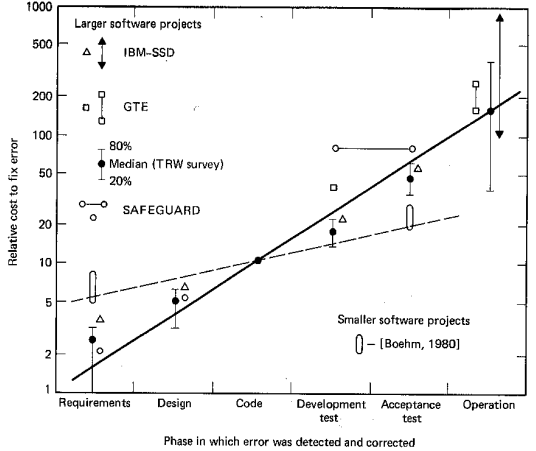
\includegraphics[width=3.3in]{boehm_cost-to-fix.png}
 \caption{Historical cost-to-fix curve. From~\cite{Boehm81}.}\label{fig:cost-to-fix}
 \end{figure}
 
In the 40 years since these initial studies, few studies have been published on the cost-to-fix curve as a function of lifecycle phase. Boehm~\cite{Boehm80} provides data suggesting that the cost-to-fix curve for small projects (from two student projects of 2000 deliverable source instructions) is flatter than for large projects (the dashed line of Figure~\ref{fig:cost-to-fix}). Shull et al.~\cite{Shull02} conducted a literature survey and held a series of e-workshops with industry experts on fighting defects. Workshop participants from Toshiba and IBM reported cost-to-fix ratios of 1:137 and 1:117 for large projects respectively~\cite{Shull02} -- the raw data points are not provided. One notable example to the traditional cost-to-fix curve is the CCPDS-R described by Royce~\cite{Royce98}: a million-line, safety-critical missile defense system (Figure~\ref{fig:royce}). In this project, design changes (including architecture changes) required approximately twice the effort of implementation and test changes, and the cost-to-fix in implementation and test phases increased slowly. Boehm~\cite{Boehm10} attributes this success to the CCPDS-R development process, which focused on removing architecture risk early in the development lifecycle.

\begin{figure}[!ht]
 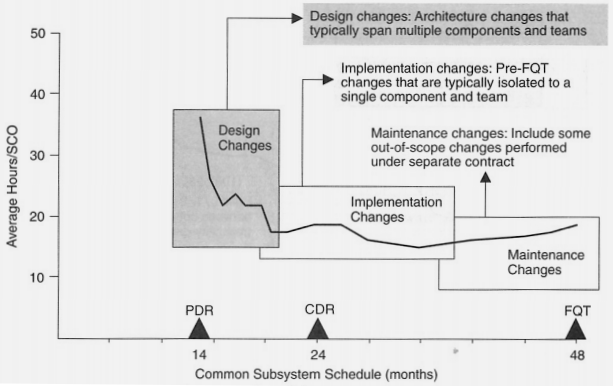
\includegraphics[width=3.3in]{Royce98.png}
 \caption{Exception to the rule - CCPDS-R case study cost-to-fix curve. From~\cite{Royce98}.}\label{fig:royce}
 \end{figure}
 
As discussed is \S\ref{sec:why-study}, one goal of agile methods is to flatten the cost-to-change curve~\cite{beck00}. Relatively little empirical data exists on this point. Clutterbuck et al.~\cite{Clutterbuck09} studied 5-month effort by a small-to-medium enterprise team developing a 71KLOEC web interface to a database application to implement 18 change requests (Figure~\ref{fig:clutterbuck}). Note that these were for new and changed user requirements, not defects. Clutterbuck et al. found the cost of change to be relatively flat until the later phases, with much of the effort spent in analysis of the change requests~\cite{Clutterbuck09}. Elssamadisy and Schalliol~\cite{Elssamadisy02} anecdotally report on the growing, high cost of rework in a 50 person, three-year, 500KLOEC Extreme Programming project as the project grew in size and complexity.

\begin{figure}[!ht]
 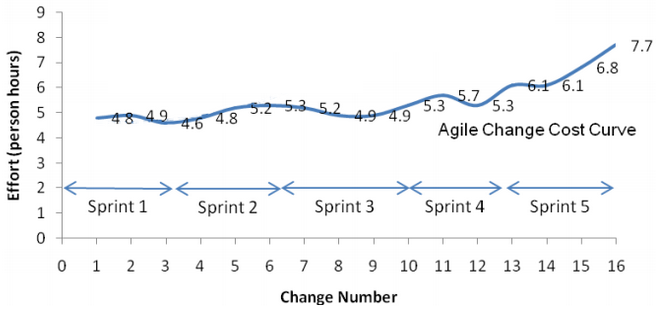
\includegraphics[width=3.3in]{clutterbuck.png}
 \caption{Cost of change from an agile case study. From~\cite{Clutterbuck09}.}\label{fig:clutterbuck}
 \end{figure}
 
 We note that previous work focuses on cost-to-fix as a function of lifecycle phase irrespective of when the defect was injected, that is, previous work analyzes the cost to fix a defect found in test regardless of whether that defect was a requirements error or a coding mistake. To our knowledge, our research represents the first large-scale study of phase delay.







%\section{carterCharts}

%anything
 

\section{Delayed Issues not  Harder\newline to Resolve}


Before presenting our analysis of phase delay in software projects, we define our terms, provide an overview of TSP and the sample projects, and describe the data collection process.

\subsection{Definitions}
A \emph{defect} is any change to a product, after its construction, that is necessary to make the product correct.  A typographical error found in review is a defect. If that same defect is discovered while writing the code but before review, it is not considered to be a defect. 

The \emph{cost-to-fix} can be computed in two ways. The first is a direct measure of the actual work time spent in correcting the defect in the product. Direct measurement enables analysis of the variability the cost-to-fix among a category of defects. The second approach measures the total time spent in a defect removal phase and divides by the total defects removed. This provides an average cost-to-fix including overhead of that activity. For example, using method two, a code inspection may require an hour of effort to remove three defects for a 3 defects per hour or to invert the ratio, 1/3 hours per defect. Most of the time, however, is spent locating the defects not actually fixing them. we use the second approach in our analysis.


\subsection{Overview of the Team Software Process}
To empirically test for the phase delay effect, we examined 171 software projects conducted between 2005 and 2014. These projects took place at organizations in many countries and were conducted using  the Team Software Process (TSP$\textsuperscript{SM}$), a software project management approach developed at the Software Engineering Institute (SEI) at Carnegie Mellon University~\cite{tsp00}. TSP is an extension of the Personal Software Process (PSP$\textsuperscript{SM}$) developed at the SEI by Watts Humphrey ~\cite{tsp00}. The data from these TSP projects were collected and stored in the Software Engineering Measured Process Repository (SEMPR) at the SEI. The Software Engineering Institute (SEI) at Carnegie Mellon University explores methods for software process improvement.
 



TSP has guiding principles; the following are relevant to this study:
\begin{itemize}
\item  Sound engineering work does not happen by accident. It must be planned.
\item  Performance of the plans requires realistic commitments of the resources needed to perform the work.
\item  The planned work should frequently be compared to  results to assure plans remain relevant.
\item  People performing the work should be responsible for planning and tracking the work.
\end{itemize}

TSP helps developers by providing a set of measures that can be applied to managing tasks, quality, and schedule. Planning begins by quantifying goals, defining work practices, and estimating size and effort. Developers then use this information to make a detailed short term plan. As the developers perform project work, they use a tool such as the Process Dashboard to collect their time, effort, size, and schedule data. Every week, the team reviews their data to evaluate status, identify actual rates, determine if project goals for schedule, cost, and quality are being met. The team then uses this information to make necessary plan corrections. At the end of the project the coach and team perform a quantitative project post mortem.

Common features of TSP projects include {\em planning}, {\em personal reviews}, {\em peer inspections}, and {\em coaching}.
A TSP {\em coach} helps the team to plan and analyze performance. The coach is the only role authorized to submit project data to the SEI.
Before reviewing data with the teams, therefore before submission, these coaches check the data for obvious errors.

{\em Planning} follows the technique taught in the PSP$\textsuperscript{SM}$. Developers estimate the size of work products and convert this to a total effort using historical rates. Time in specific tasks come from the  process phases and historical percent time in phase distributions. Defects are estimated using historical phase injection rates and phase removal yields. Coaches help the developers to compare estimates against actual results. In this way, developers acquire a more realistic understanding of their work behavior, performance, and schedule status.

{\em Personal review} is a technique taken from the PSP and its use in TSP is unique.  Developers follow a systematic process to remove defects by  examining their own work products using a checklist built from their personal defect profile. This personal review occurs after some product or part of a product is considered to be constructed and before peer reviews or test. 

%PSPSM teaches developers howto continually make and review their personnel estimates
%about their day-to-day tasks, then compare those estimates against the actual development effort.
%In this way, developers can acquire a more realistic understanding of their work behaviour.
  
 
{\em Peer inspection} is a  technique in
traditional software engineering and is often called peer review.
 Basili and Boehm   commented in 2001~\cite{boehm01} 
that peer reviews can catch over half the defects introduced into a system.
Peer inspection can be conducted on any artifact generated anywhere in the software
lifecycle and can quickly be adapted to new kinds of artifacts. TSP peer reviews follow the Fagan style in which the reviewer uses a checklist composed of common team defects prior to a review team meeting. 


\begin{figure}[!t]  
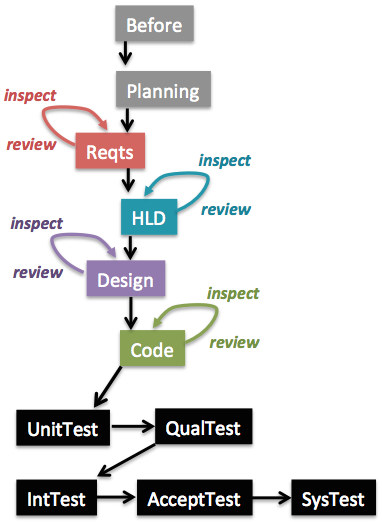
\includegraphics[width=4in]{img/waterfall-v3.png}  
\caption{Different approaches to software development:  waterfall and agile (bottom left).}
\label{fig:waterfall}
\end{figure}


\subsection{Projects in the Sample}
Since shortly before the year 2000, the SEI has been teaching and coaching TSP teams. One of the authors (Nichols) has been been mentoring software development teams and coaches around the world as they deploy TSP within their organizations since 2006.  The  most recent completions were in 2014.
The projects were mostly small to medium, with a median duration of 46 days and a maximum duration of 90 days in major increments. 
Several projects extended for multiple incremental development cycles. 
Median team size was 7 people, with a maximum of 40. 

Many of the projects were e-commerce web portals or banking systems in the US, South Africa, and Mexico. 
There were  some  medical device projects in  the US, France, Japan, and Germany as well  as a commercial computer-aided design systems, and embedded systems. 

An anonymized version of that data is available in the PROMISE repository\footnote{http://openscience.us/repo}  and,
for confidentiality restrictions, we cannot offer 
further details on these projects.



\subsection{Data Collection Process}
\label{sec:data-collection}

Organizations using TSP agree to provide their project data to the SEI for use in research. In return the SEI agrees    that  data must not be traceable to its source. The data is collected at major project events; launch, interim checkpoints, and at project completion. Data includes project and site  characteristic summaries, surveys of team members, launch presentations, launch outbriefs, and baseline plans, final data from the project, and the project post mortem report.  In practice, this data requirement has only been enforced for the purposes of certifying and reauthorizing TSP coaches who must submit data to maintain their authorization. Coaches are certified by demonstrating competent use of the TSP process with the artifacts and data not by the actual project results.  Of the data submitted, only the data recorded using the Process Dashboard tool has been collected and aggregated for this research. 

To use this data for research and benchmarking,  Nichols first collected the Process Dashboard data from the submission repository then used a tool built by the Process Dashboard developer, David Tuma, 
to gather the project data into a database. Nichols and his colleague Yasutaka Shirai then extracted data into views suitable for analysis. The key views include a project results summary, effort logs, task logs, and defect logs. The data has not yet undergone additional screening. A summary of the data quality issues was reported in a previous work ~\cite{shirai14} (that summary is discussed further in our {\em Validity} section, below).

The tool collected process information about those tasks and defects that we analyze in this work. 
That task data include  work start time, work end time, delta
work time, and interruption time. Software engineers are often
interrupted by meetings, requests for technical help, reporting, and
so forth. These events are recorded, in minutes, as interruption
time. 

 Defect logs include the time and date a defect was discovered, the phase in which that defect was injected, the phase in which it was removed, the time (in minutes) required to find and fix the defect, and the categorical type.

The defect types in the most common defect type standard  in the the SEI TSP data are follows:
\begin{itemize}
\item Environment: design, compile, test, or other support system problems
\item Interface: procedure calls and reference, I/O, user format
\item Data: structure, content
\item Documentation: comments, messages
\item Syntax: spelling, punctuation typos, instruction formats
\item Function: logic, pointers, loops, recursion, computation, function defects  
\item Checking: error messages, inadequate checks
\item Build: change management, library, version control
\item Assignment: package
declaration, duplicate names, scope, limits
\item System: configuration, timing, memory
\end{itemize}


As of November 2014, the SEI TSP database contained data from 212
TSP projects. The projects completed between July 2006 and
November 2014; they included 47 organizations and 843 people. 
The database fact tables
contain 268,726 time logs, 
154,238 task logs,
 47,376 defect logs, 
and 26,534 size logs. 
After selecting defects from the data log and joining the data to the time log table  171 of these projects remained. The excluded projects had no or too few defects to use in this analysis.
 
In this paper, when we report ``time to resolve an
issue,'' we show the difference between the start and end times
of a work session, with any interruption time subtracted (the
difference in times, minus the interruptions). 


%That said, certain semantic features of the SEI TSP data should be noted.
%Firstly, in the current TSP collection tool, 
%fix times are only the developer time for the developer walking through the phases of \fig{waterfall}.
%We are currently tracking the fix time for post-release issues (e.g. those raised during  acceptance test and %later
%product life cycle). So far, in that post-release data,  we have not detected
%a dramatic phase escalation effect (but at this time, we have nothing definitive comment on that matter).%
%
%\bill{somewhere you have one note on \underline{find} and fix times.  for this paper, we need just fix times. %but is there
%anything we need to fret about re \underline{find} times?}
 
 

\subsection{Project Phases}
This paper studies the impact of phase delay on the time required to resolve issues.
The logical phases used in this paper are shown in \fig{waterfall}. Although the representation suggests a waterfall, the phases represent the primary stages through which requirements are developed into working and tested code. That is, all requirements must be stated in some way, implemented in code, integrated, and tested. All real implementations of any size follow a spiral approach with many team performing the work in iterative and/or incremental development cycles.  Within a project increment, multiple features or components may be developed and incremented. TSP is compatible with agile and encourages iterative and incremental development. Nonetheless, the specific strategy and cycle duration is a project decision. TSP does, however, strongly encourage 1) constructing units of sufficient size that measurement is practicable, and 2) separating the construction from appraisal and test activities. This effectively highlights the separation of construction from rework activities and aids the apportionment of defects to those found in appraisal activities (reviews and inspections) and those found through failure (test). The distinct construction activities (requirements, high and detailed design, and code) were chosen to help teams analyze the effectiveness and efficiency of their practices through analysis of the defect phase origin, type, fix effort, and phase of discovery. 

Note that, in that Figure~\ref{fig:waterfall}:
\bi 
\item
Several  phases in which product is created have sub-phases of {\em review} and {\em inspect} to remove defects. TSP uses review, a sub-phase in which individuals perform personal reviews of their work products prior to the peer review, which TSP calls the inspection.
\item Testing is divided into several stages. Developers perform unit test prior to code complete.  After code complete a standard phase is the integration, which combines program units into workable system ready for system test. Integration,  system test, and acceptance test are often performed by a separate group. 
\ei
For these TSP projects, the principles followed are: 
\bi 
%\item Defects should be found before test, that is, test defects should be infrequent.
\item A product should be inspected before used in a subsequent construction phase to minimize  unnecessary rework.
\item To minimize unnecessary rework, a product should be reviewed and inspected prior to use in a subsequent construction phase.
\item A personal review should remove the most common defects before being given to peers for the inspection.
\item Because different categories of test will find different types of defect, and follow in a natural sequence, the tests should be measured separately
\ei 
In summary, the TSP process and measurement have been specifically designed to aid the analysis of defects for use in process improvement. The data are, therefore, uniquely suitable for an analysis of the phase delay effect. 
\subsection{Distinguishing Project Characteristics}
Modern development processes include the core engineering practices of estimation, planning, configuration control, requirements, design, code development, and test. Agile methods address  not only these core practices but also address team organization, individual and team commitments, test and build automation, and implementing iterative and incremental development. TSP uses additional practices associated with high performance ~\cite{jones10} including; project tracking and control, specialization of team members, inspections, static analysis, documentation and training, and reuse. Although the teams in this sample use many typical agile practices, they are also using additional practices. 



Using the above,
our units of analysis are:
\bi
    \item \emph{defects} - individual defects are recorded as line items in the defect logs uploaded to the SEMPR at the SEI. One or more defects are reported against a single \emph{plan item} in the time tracking logs, e.g., a review session, an inspection meeting, a test execution.
    \item \emph{time} - Time is tracked per person per plan item in the time-tracking logs, e.g. a 30 minute design review session involving 3 people will have three time log entries summing to 90 minutes. Time includes the time to analyze, repair, and validate a defect fix.
    \item \emph{time per defect} - The total \# of defects found in a plan item during a removal phase divided by the total time spent on that plan item in that phase.
\ei


%\todo{
%\bi
%    \item What is the cost-to-fix curve in TSP data? Check against H1 and compare to past literature.
%    \item What is the effect of phase delay? Check against H2.
%    \item \fig{cost-to-fix-tsp} is great. really important. its from  different decades, right?  so can we add text saying that the general pattern is that the (approx) 15 years between each curve tends to a flattening. not, perhaps, due to process but to better build environs.
%\ei
%}

 
 

\begin{figure}[!t] 

%\hspace{-0.7cm}
\begin{center}
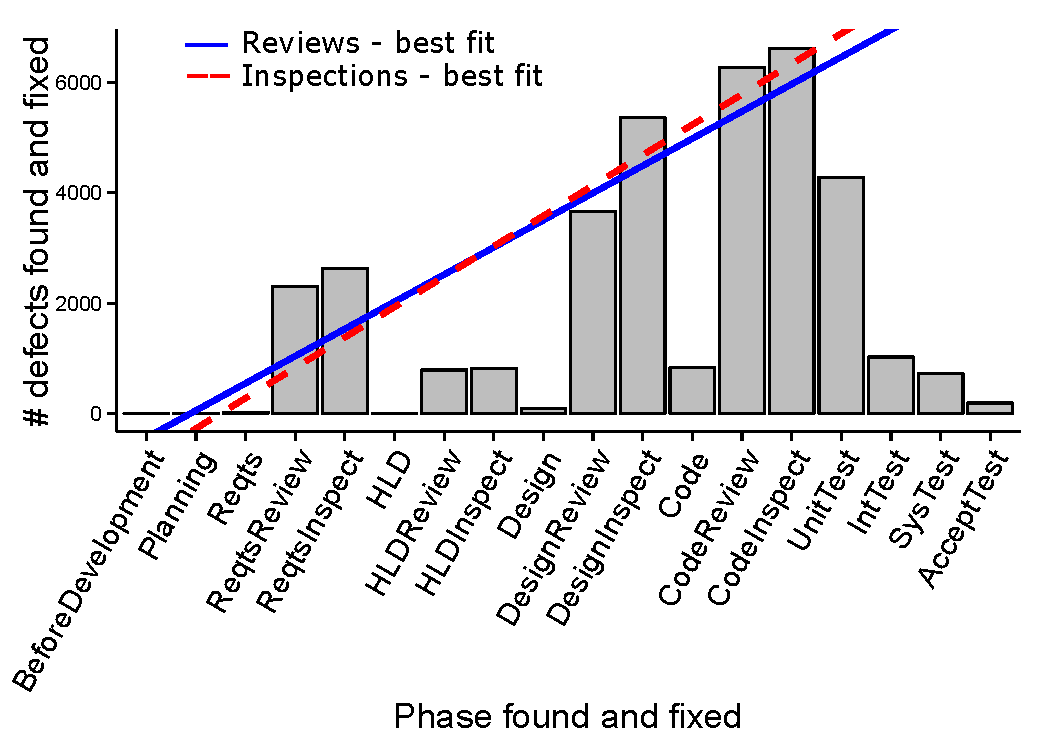
\includegraphics[height=2in]{img/fix-phase-dist.pdf}
\end{center}
%~\\

\caption{Distribution of defects found and fixed by phase.}
\label{fig:fix-phase-dist}
\end{figure}


\begin{figure}[!t] 
 \renewcommand{\baselinestretch}{0.7}
 \scriptsize
\begin{center}
\begin{tabular}{r@{~}|r@{~}r@{~}r|@{~}l@{~}l|@{~}r@{~}l}  % I attach your cursor. thrust, parry, yo!
  \multicolumn{1}{c}{~} &\multicolumn{3}{c}{Percentiles}&\multicolumn{2}{l}{~~~~~~Phase}\\%\cline{2-6}
N & 25th & 50th & 75th &   injected & removed   & \multicolumn{2}{l}{Scale up w.r.t. to first phase}\\\hline
\\
 48&   14&   30&   51&Before&DesignInspect &1.00 & **********  \\
 53&   13&   28&   49&Before&CodeReview &0.93 & **********  \\
 94&   22&   45&   80&Before&CodeInspect &1.50 & ***************  \\
153&   38&   77&  130&Before&UnitTest &2.56 & **************************  \\
127&   30&   65&  128&Before&IntTest &2.16 & **********************  \\
 92&   24&   56&   89&Before&SysTest &1.86 & *******************  \\
 
 
\\
 56&   14&   35&   57&Planning&ReqtsReview &1.00 & **********  \\
 46&   11&   24&   39&Planning&DesignInspect &0.68 & *******  \\
 32&   18&   33&   84&Planning&UnitTest &0.94 & **********  \\
 
\\
184&   45&   92&  155&Reqts&ReqtsReview &1.00 & **********  \\
189&   46&   93&  155&Reqts&ReqtsInspect &1.00 & **********  \\
 61&   14&   33&   55&Reqts&DesignReview &0.35 & ****  \\
102&   24&   49&   83&Reqts&DesignInspect &0.52 & ******  \\
 59&   18&   38&   60&Reqts&CodeInspect &0.40 & ****  \\
 91&   22&   49&  104&Reqts&UnitTest &0.52 & ******  \\
100&   33&   67&  120&Reqts&IntTest &0.72 & ********  \\
 78&   28&  122&  237&Reqts&SysTest &1.31 & **************  \\
\\
210&   51&  103&  166&Design&DesignReview &1.01 & ***********  \\
207&   50&  101&  156&Design&DesignInspect &1.00 & **********  \\
134&   32&   66&  116&Design&CodeReview &0.65 & *******  \\
163&   39&   79&  135&Design&CodeInspect &0.78 & ********  \\
238&   58&  119&  183&Design&UnitTest &1.17 & ************  \\
172&   42&   88&  158&Design&IntTest &0.87 & *********  \\
163&   40&   80&  161&Design&SysTest &0.79 & ********  \\
 80&   21&   45&   73&Design&AcceptTest &0.44 & *****  \\
 
\\
235&   57&  115&  177&Code&CodeReview &1.00 &  **********  \\
228&   56&  113&  176&Code&CodeInspect &0.99 & ********** \\
243&   59&  125&  206&Code&IntTest &1.08 &     *********** \\
191&   46&   95&  173&Code&SysTest &0.82 &     ******** \\
269&   66&  133&  206&Code&UnitTest &1.15 &    ***********  \\
130&   31&   65&  122&Code&AcceptTest &0.56 &  ******  \\
 \end{tabular}
\end{center}
\caption{Distribution of fix times seen in SEI TSP data. Left hand side bars
show scale up on median values.
}
\label{fig:raw}
\end{figure}



\subsection{Observations from 171 Projects}

The distribution of defects found and fixed per phase in our data is shown in Figure~\ref{fig:fix-phase-dist}. A high percentage of defects (44\%) were found and fixed in the early phases, i.e., requirements, high level design, and design reviews and inspections. (This distribution is similar to that observed for other projects that emphasized investment in software engineering quality assurance practices. For example, Jones and Bonsignour report 52\% of pretest defects removed before entering implementation, for large projects that focus on upfront defect removal techniques \cite{jones12}. NASA robotics projects had a slightly higher percentage (58\%) of defects removed before implementation began, although these had invested in IV\&V on top of other forms of defect removal \cite{me08a}.)  

\fig{raw} shows the 25th, 50th, 75th percentile
of the time spent on {\em review} or {\em inspect} or {\em test} phases
in our 171 projects.
Note that, in TSP, when developers see issues, they enter {\em review} or 
{\em inspect} or {\em test}
until that issue is retired.

In that figure, the data is split out according to issues that were fixed in phase $Y$ after
being introduced in phase $X$. The data is sub-divided into tables according to $X$;
i.e. according to {\em before, planning, requirements, design} or {\em  code}. 
The stars on the right-hand-side of that figure show the scale ups associated with the phase removal stages,
expressed as a ratio of the first item in that block (which, by definition, is 1.00 for
that first item).
If  this data exhibited a delayed issue effect,  we would expect those bars in each sub-division to exhibit an
exponential shape.

\subsubsection{Comment 1}
Figure~\ref{fig:fix-phase-dist}
 data does not support   
{\em  requirements errors are the most expensive to fix}.
Note that   median time spent fixing errors from {\em requirements} across the life cycle was 92, 93,  49, 33, 39, 49, 67, 122 minutes\footnote{If this time seems long, then recall
that it includes the time required  to (a)~collect data and realize there is an error;
(b)~prepare a fix;  and (c)~apply some validation
procedure to check the fix (e.g. discuss it with a colleague or execute some tests).}.
This is:
\bi
\item
Clearly longer than median times seen {\em Before } and in {\em Planning}
(30,28,45,77,65,56,24,35,33);
\item
Somewhat shorter, but still not exponentially smaller,  than the median times see after {\em requirements} in {\em design}
(103,101, 79,66, 119,88, 80,45) and in {\em code} (65,115, 113,125, 95,133). 
\ei
For completeness, we ran an  
A12 test comparing the raw data (and not just the medians of \fig{raw}) and found
 a non-small effect only for the difference {\em requirements}
to {\em code}. But even though the effect was non-small, 
 the overall size of the difference
{\em requirements} to {\em code} was less than 30\% (i.e. much less than we would
expect from the delayed issue effect). 

That said, Figure~\ref{fig:fix-phase-dist} does support the 
claim that early lifecycle errors are most expensive to fix.
In all our results, the biggest scale ups are found with resolving
issues introduced in the {\em before} phase. For example,
resolving {\em before} issues during unit testing was 2.56 times
slower than resolving issues earlier in the lifecycle. 

Nevertheless,  it must be added that the scale up seen in 
Figure~\ref{fig:fix-phase-dist} 
is much less
than suggested by the DIE literature. Returning to
the {\em before/unit test} result: 2.56 is far smaller
than the scale ups seen in Figure~1. In fact, nowhere in 
our results do we see any exponential increase.

\subsubsection{Comment 2}
Next, we comment on 
requirements errors are the most expensive to fix 
{\em when found during production but the cheapest to fix early in development}. 
Our data from these 171 project does not extend into post-delivery deployment. That said,
there is enough evidence to raise doubts that our projects will exhibit exponentially more
difficult issues after deployment. 

That evidence is as follows.
Prior reports of an  exponential increase in difficulty in resolving issues {\em during
development}.
For example:
\bi
\item  From requirements to acceptance testing
\fig{b81} reports a 40-fold increase;
\item
 \fig{cost-to-fix} reports a 100-fold increase
(for the larger projects).
\item
The projects surveyed in \fig{steck} report changes of a  \newline
\{37,40,40,50,51,70,75,250\}-fold increase in pre-deployment period when the software was being developed.
\ei
Any manager watching  these intra-development trends would be well-justified
to anticipate that  the difficulty in resolving issues would will get much worse. Such managers
would therefore expect an exponentially harder time resolving issues during deployment.

On the other hand, a remarkable feature of Figure~\ref{fig:fix-phase-dist} is the {\em absence}
of an exponential delay effect during development.
In our data, the greatest difficulty in resolving requirements issues was 1.31 seen in systems testing--
which is far smaller than the 37 to 250-fold increases reported in \fig{b81}, \fig{cost-to-fix},
and \fig{steck}.  That is, from our  data, we would not anticipate exponentially greater difficulty in resolving requirements issues after
deployment. 
 \subsubsection{Comment 3}
 The above specific statements related just to requirements. Turning now
 to issues creased in all phases in Figure~\ref{fig:fix-phase-dist},  we see that
 this data does not follow the exponential increase predicted
by the delayed issue effect:
\bi
\item There is much ``up and down'' in the chart. 
\item If we separate out just the {\em Inspect} or {\em Review} data, we can see that there is some increase in {\em Design} and {\em Code}. However, that effect could be a linear or be just noise. In either case,
it does not look like exponential.
\item The time in final testing is particularly low suggesting that few defects survived into testing
(and hence, there were few instances where code required massive rework).
\ei
In summary:
\bi
\item
The delayed issue effect has been reported in around a dozen papers, at least half of which date back to the 1970s. 
\item
But there is no trace of that  effect   in hundreds of software projects built  since 2006.
\ei
%For illustrative purposes, the relative cost to fix errors per lifecycle phase in the TSP project data is overlayed with Boehm's cost curve~\cite{Boehm81} as well as the CCPDS-R case study~\cite{Royce98} in \fig{cost-to-fix-tsp}. Cost-to-fix for TSP is total time spent in each review, inspection, or test-related phase / \# of defects found in phase (reported in \fig{raw}). It is clear to see that the trend is relatively flat, closer to the pattern exhibited by the Royce case study (which also focused on early defect removal) than the exponential growth curve.
 


%\begin{figure}[!t] 
%%\vspace{-1cm}
%\hspace{-0.35in}
%\begin{center}
%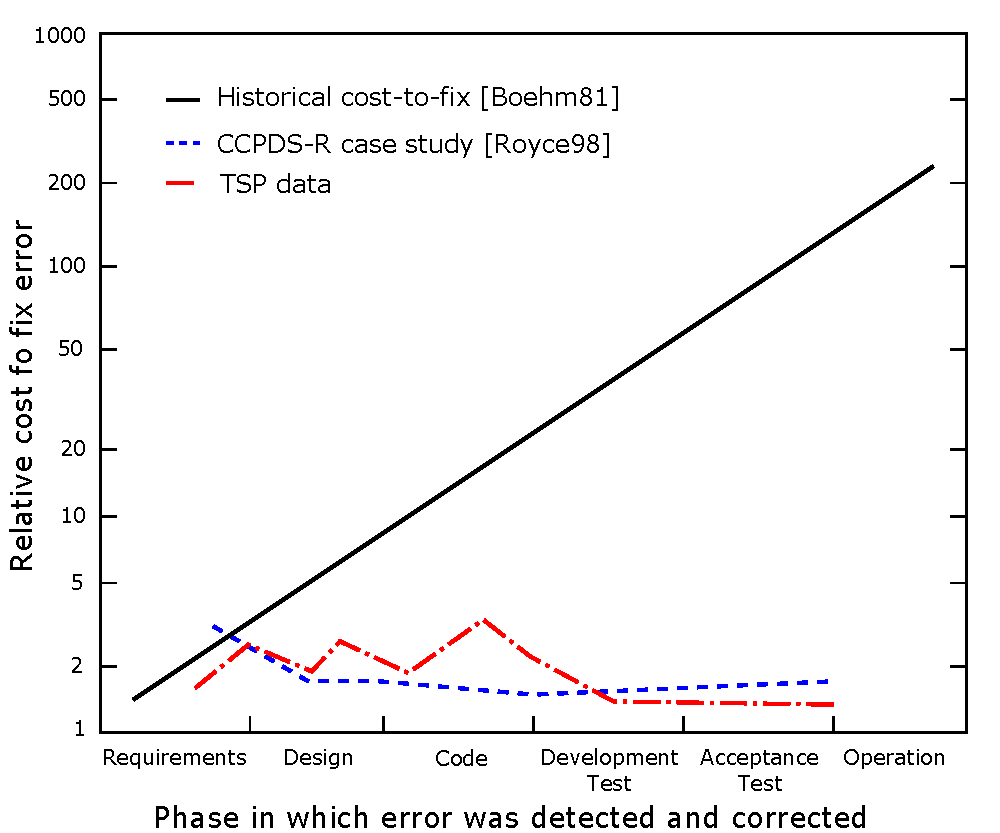
\includegraphics[width=3in]{img/boehm-overlay.pdf}
 %\end{center}
% ~\\~\\
%~\\~\\~\\
 
 %\caption{Cost-to-fix curve from \protect\fig{cost-to-fix} 
 %overlayed with case study from~\cite{Royce98} and TSP data. Scale is relative to the phase with the lowest %c%ost to fix. }\label{fig:cost-to-fix-tsp}
% \end{figure}
 
%\begin{table}[ht]
%\renewcommand{\baselinestretch}{0.7}
% \scriptsize
%\centering
%\begin{tabular}{ll|ll}
%  Phase num & Name & \# defects & percentage \\ 
%  \hline
%1 & BeforeDevelopment &   0 & 0.00 \\ 
%  2 & Planning &   4 & 0.00 \\ 
%  3 & Reqts &  25 & 0.10 \\ 
%  4 & ReqtsReview & 2304 & 6.50 \\ 
%  5 & ReqtsInspect & 2630 & 7.40 \\ 
%  6 & HLD &   0 & 0.00 \\ 
%  7 & HLDReview & 790 & 2.20 \\ 
%  8 & HLDInspect & 818 & 2.30 \\ 
%  9 & Design &  94 & 0.30 \\ 
%  10 & DesignReview & 3668 & 10.30 \\ 
%  11 & DesignInspect & 5365 & 15.00 \\ 
%  12 & Code & 833 & 2.30 \\ 
%  13 & CodeReview & 6276 & 17.60 \\ 
%  14 & CodeInspect & 6623 & 18.60 \\ 
%  15 & UnitTest & 4283 & 12.00 \\ 
%  16 & IntTest & 1024 & 2.90 \\ 
%  17 & SysTest & 730 & 2.00 \\ 
%  18 & AcceptTest & 189 & 0.50 \\ 
% \end{tabular}
%\caption{Defects found per phase} 
%\label{fig:defect_per_phase}
%\end{table}



%\begin{figure}[!ht]
%
% \renewcommand{\baselinestretch}{0.7}
% \scriptsize
%\begin{center}
%\begin{tabular}{r|rr|rl}
%Phase & samples & total time&\multicolumn{2}{l}{Total time w.r.t. first phase}\\\hline
%~\\
%Planning&229&12625&1.00&*\\
%~\\
%Reqts&590&24182&1.91&**\\
%ReqtsInspect&2533&92723&7.34&********\\
%ReqtsReview&1762&67471&5.34&******\\
%~\\
%HLD&78&6856&0.54&*\\
%HLDReview&472&12821&1.01&**\\
%HLDInspect&1366&35291&2.79&***\\
%~\\
%Design&620&21573&1.70&**\\
%DesignInspect&8373&229937&18.21&*******************\\
%DesignReview&3043&92823&7.35&********\\
%~\\
%Code&3029&220058&17.43&******************\\
%CodeReview&4774&163091&12.91&*************\\
%CodeInspect&11406&334442&26.49&***************************\\
%~\\
%UnitTest&9177&352245&2.790&****************************\\
%IntTest&2761&160559&12.71&*************\\
%SysTest&2059&105796&8.37&*********\\
%AcceptTest&1045&42717&0.338&****\\
%\end{tabular}
%\end{center}
%\caption{Times per phase (minutes).}
%\label{fig:fix-time-per-phase}
%\end{figure}



%we calculate phase delay as simply the number of project phases (the set used in our data set is shown in %\fig{waterfall}) during which the defect existed in the system, i.e. the ordinal rank of removal phase minus the %ordinal rank of injection phase. Sub-phases (such as review and inspection) are included in this calculation.
%


 
 %\begin{figure}[!t]
%\%renewcommand{\baselinestretch}{0.7}
%\scriptsize
%\begin{center}
%\begin{tabular}{l@{~~}|l@{~}|r@{~}|r@{~}r@{~}|r@{~}l}
%%           \multicolumn{2}{c}{~}                 &  &\multicolumn{2}{c|}{median}\\
 % Injection&   Removal& $n$ & initial & now & \multicolumn{2}{l}{Scale up, w.r.t. initial}
%\\\hline

BeforeDevelopment&Code.dat&57&1&\rule{2mm}{2mm} \\
BeforeDevelopment&CodeInspect.dat&72&0.3&\rule{0mm}{2mm} \\
BeforeDevelopment&Test.dat&165&1.1&\rule{2mm}{2mm} \\
BeforeDevelopment&IntTest.dat&50&1.3&\rule{2mm}{2mm} \\
BeforeDevelopment&SysTest.dat&42&1.8&\rule{2mm}{2mm} \\
\\\hline

Planning&Planning.dat&66&1&\rule{2mm}{2mm} \\
Planning&ReqtsReview.dat&41&0.8&\rule{0mm}{2mm} \\
\\\hline

Reqts&Reqts.dat&23&1&\rule{2mm}{2mm} \\
Reqts&ReqtsReview.dat&245&13&\rule{26mm}{2mm} \\
Reqts&ReqtsInspect.dat&289&16&\rule{32mm}{2mm} \\
Reqts&Design.dat&32&21&\rule{42mm}{2mm} \\
Reqts&DesignInspect.dat&49&7&\rule{14mm}{2mm} \\
\\\hline
 

HLD&HLDReview.dat&94&1&\rule{2mm}{2mm} \\
HLD&HLDInspect.dat&133&1.6&\rule{2mm}{2mm} \\
HLD&Design.dat&33&1&\rule{2mm}{2mm} \\
\\\hline

Design&Design.dat&37&1&\rule{2mm}{2mm} \\
Design&DesignInspect.dat&455&6&\rule{12mm}{2mm} \\
Design&Code.dat&218&3.5&\rule{6mm}{2mm} \\
Design&CodeInspect.dat&166&2.7&\rule{4mm}{2mm} \\
Design&Test.dat&542&7.7&\rule{14mm}{2mm} \\
Design&IntTest.dat&67&3.7&\rule{6mm}{2mm} \\
Design&SysTest.dat&92&6.3&\rule{12mm}{2mm} \\
\\\hline

DesignInspect&DesignInspect.dat&53&1&\rule{2mm}{2mm} \\
DesignInspect&Code.dat&38&0.75&\rule{0mm}{2mm} \\
\\\hline

Code&Code.dat&126&1&\rule{2mm}{2mm} \\
Code&CodeInspect.dat&459&2&\rule{4mm}{2mm} \\
Code&Test.dat&461&2.16667&\rule{4mm}{2mm} \\
Code&IntTest.dat&348&2.16667&\rule{4mm}{2mm} \\
Code&SysTest.dat&230&1.5&\rule{2mm}{2mm} \\
Code&AcceptTest.dat&71&0.916667&\rule{0mm}{2mm} \\
\\\hline

CodeInspect&CodeInspect.dat&64&1&\rule{2mm}{2mm} \\
CodeInspect&Test.dat&57&1.25&\rule{2mm}{2mm} \\
\\\hline

Test&Test.dat&110&1&\rule{2mm}{2mm} \\
Test&QualTest.dat&66&0.4&\rule{0mm}{2mm} \\
\\\hline

IntTest&QualTest.dat&32&1&\rule{2mm}{2mm} \\
IntTest&IntTest.dat&36&5.5&\rule{10mm}{2mm} \\
IntTest&SysTest.dat&21&1&\rule{2mm}{2mm} \\ 
%\end{tabular}
%%\end{center}
%\caption{50th percentile (median) scale ups  for  time to resolve issues (taken from \fig{raw}).}
%%\label{fig:scale}
%\end{figure}
 



 


%\subsection{Phase Delay in Slower Bugs?}
%In these results, we checked if a small number of bugs are most expensive. 
%To check this:
%\bi
%\item
%We repeated the analysis that generated \fig{scale},
%but instead of looking at the 50th percentile, we displayed the scale up factors
%\item 
%We only
%checked the Design and Code scale up results since, from \fig{scale}, it is clear these
%have the most examples of longest phase delays.
%\ei 
%The  results are shown in \fig{scale90} and these
%results are somewhat different for Design and Coding issues: 
%\bi 
%\item For Design issues,  these have the same
%general form as the 50th percentile results. That is, while it it certainly faster
%to remove thing sin the phase where they are created, once we leave that phase
%it does not seem to matter much how many phases we wait before fixing the issue.
%\item
%\item For Coding issues, the seems little impact of phase delay on the time
%required to fix.
%\ei

 


%\begin{figure}[!t]
%\renewcommand{\baselinestretch}{0.7}
%\scriptsize
%\begin{center}
%\begin{tabular}{l@{~~}|l@{~}|r@{~}|r@{~}r@{~}|r@{~}l}
%          \multicolumn{2}{c}{~}                 &  &\multicolumn{2}{c|}{99th }\\
%           \multicolumn{2}{c}{~}                 &  &\multicolumn{2}{c|}{percentile }\\
%  Injection&   Removal& $n$ & initial & now & \multicolumn{2}{l}{Scale up, w.r.t. initial}
%\\\hline

B4dev&Code&57&257&257&1&\rule{2mm}{2mm} \\
B4dev&CodeInspect&72&257&153&0.60&\rule{2mm}{2mm} \\
B4dev&Test&165&257&282&1.093&\rule{2mm}{2mm} \\
B4dev&IntTest&50&257&365&1.42&\rule{2mm}{2mm} \\
B4dev&SysTest&42&257&151&0.59&\rule{2mm}{2mm} \\

\\\hline

Design&Design&37&600&600&1&\rule{2mm}{2mm} \\
Design&DesignInspect&455&600&277&0.46&\rule{0mm}{2mm} \\
Design&Code&218&600&240&0.4&\rule{0mm}{2mm} \\
Design&CodeInspect&166&600&163&0.27&\rule{0mm}{2mm} \\
Design&Test&542&600&652&1.09&\rule{2mm}{2mm} \\
Design&IntTest&67&600&277&0.46&\rule{0mm}{2mm} \\
Design&SysTest&92&600&480&0.8&\rule{2mm}{2mm} \\

\\\hline

Code&Code&126&600&600&1&\rule{2mm}{2mm} \\
Code&CodeInspect&459&600&243&0.41&\rule{0mm}{2mm} \\
Code&Test&461&600&365&0.61&\rule{2mm}{2mm} \\
Code&IntTest&348&600&7200&12&\rule{24mm}{2mm} \\
Code&SysTest&230&600&290&0.48&\rule{0mm}{2mm} \\
Code&AcceptTest&71&600&600&1&\rule{2mm}{2mm} \\
%\end{tabular}
%\end{center}
%%\caption{99th percentile scale ups.}
%\label{fig:scale99}
%\end{figure}

%\begin{figure}[!t]
%\renewcommand{\baselinestretch}{0.7}
%\scriptsize
%\begin{center}
%\begin{tabular}{l@{~~}|l@{~}|r@{~}|r@{~}r@{~}|r@{~}l}
 %          \multicolumn{2}{c}{~}                 &  &\multicolumn{2}{c|}{mean}\\
 % Injection&   Removal& $n$ & initial & now & \multicolumn{2}{l}{Scale up, w.r.t. initial}
%\\\hline

B4dev&Code&57&34&34&1&\rule{2mm}{2mm} \\
B4dev&CodeInspect&72&34&12&0.35&\rule{0mm}{2mm} \\
B4dev&Test&165&34&39&1.15&\rule{2mm}{2mm} \\
B4dev&IntTest&50&34&37&1.09&\rule{2mm}{2mm} \\
B4dev&SysTest&42&34&46&1.364&\rule{2mm}{2mm} \\
\\\hline
  

Design&Design&37&21&21&1&\rule{2mm}{2mm} \\
Design&DesignInspect&455&21&41&1.958&\rule{4mm}{2mm} \\
Design&Code&218&21&28&1.33&\rule{2mm}{2mm} \\
Design&CodeInspect&166&21&20&0.95&\rule{2mm}{2mm} \\
Design&Test&542&21&59&2.81&\rule{6mm}{2mm} \\
Design&IntTest&67&21&42&2&\rule{4mm}{2mm} \\
Design&SysTest&92&21&42&2&\rule{4mm}{2mm} \\
\\\hline
 

Code&Code&126&48&48&1&\rule{2mm}{2mm} \\
Code&CodeInspect&459&48&38&0.79&\rule{2mm}{2mm} \\
Code&Test&461&48&52&1.08&\rule{2mm}{2mm} \\
Code&IntTest&348&48&379&7.90&\rule{16mm}{2mm} \\
Code&SysTest&230&48&37&0.77&\rule{2mm}{2mm} \\
Code&AcceptTest&71&48&30&0.63&\rule{2mm}{2mm} \\


%\end{tabular}
%\end{center}
%\caption{Mean  scale ups.}
%\label{fig:scale90}
%\end{figure}


 


 
 

\section{Validity}
We report validity concerns following the guidelines of Runeson \& H\"{o}st~\cite{runeson09}.

\subsection{External validity}
Threats to external validity affect the generalization of findings. The most obvious threat to external validity is that TSP is not representative of most software development processes. Hence,
For example, 
one way to discount the above is that our sample is biased-- that while general software
systems suffer from the delayed issue effect, systems built using TSP are so much better controlled
that they  mitigate against the DIE effect.

It would be convenient to offer the last paragraph as the conclusion of this study
(two of our authors, Nichols and Shull,  work at the organization that invented and promoted TSP).
 However, we cannot endorse such a conclusion:
 \bi
 \item
We view TSP as a better way to
 {\em monitor} the activities {\em of  existing projects}. That is, TSP
 does not radically change a project, it just offers a better way to log the activity within
 that project. 
 \item
 Our 171 project contain examples of a wide variety
 of systems (e-commerce web portals and  banking systems) run in a variety of
 ways (agile or  waterfall or some combination of the two). Hence, rather
 than being unduly  biased in some manner,
 we view our 171 projects as a large sample of current industrial processes for software
 development.
 \ei
Another way to discount this result is to say we are only reporting on small to medium-size
projects, and the real impact of delayed issues is on very large projects.
There certainly exists another class of very large software project where early requirements
errors would be catastrophic for later development. For example, when NASA launches deep space missions,
each of those satellites are special-purpose, uniquely-built devices built by a large contractor
population. Such systems are very hard to reconfigure halfway through the development.  

We concede that for very large complex NASA-like developments, the delayed issue
effect could still hold. However, perhaps we need to split our software engineering principles
into two parts- one for   very large NASA-like projects (which are not very numerous)
and one for smaller-sized projects like the ones studied here (which are far more numerous).
Most software is {\em not} like the software used on NASA deep-space satellites.
As  agile methods grew more popular last decade; and as personnel computers grew more powerful;
and as the libraries associated with particular languages grew more extensive; then smaller
teams starting  deliver systems that (previously) had required very large teams.
As mentioned above,
our  171 projects represents $\frac{171}{212}=80$\% of the software projects
seen by the Software Engineering Institute. That is, as far as we can tell,
there are more small to medium-sized projects than otherwise.


\subsection{Construct validity} 

Our definition of {\em difficult to resolve} combines two concepts: time to change and cost to
change. In the above we have used them interchangable, comparing our time to resolve data (from the 171 TSP projects) against the cost-to-fix results of Boehm et al. e.g. \fig{b81}.
Is it valid to assume the equivalence of time and cost?

Certainly, there are cases where time is not the same as cost. Consider, for example,
if debugging required some very expensive tool or the services or a very senior (and hence, very expensive)
developer. Under those circumstances, time does not equate to cost.

Also, there is the issue of the implication of  a defect. Evidence discussed in \cite{Shull02} suggests that low severity defects may exhibit a lower cost to change. Nonetheless, even ``small'' typographical errors have been known to cause enormous damage (e.g., the Mars climate Orbiter). 

Having documented the above issues, we assert that they are probably not major issues in the study.
As to the first point, that some debugging may be more expensive than others, one of us (Nichols)
was closely associated with many of the projects in our sample. He is unaware of any frequent
use of exorbitantly expensive tools or people on these projects. As to the second point (that
some defects have an impact beyond the mere cost to fix them), we no evidence suggesting
that the net effect of this concern over all our projects is non-zero.


\subsection{Internal validity}
Confounding variables are a threat to any study. In this research, we rely on the substantial sample size of 171 TSP projects and over 47,000 defect logs to avoid confounding effects that may arise from the nature of the projects, teams, or defects. Similarly, the 10-year data collection period should help to ameliorate any maturation or history effects.  As described in \S\ref{sec:data-collection}, all TSP teams are required to contribute time and defect data to the SEI, and thus there should be no selection bias in this sample compared to the overall population of TSP projects. However, there is likely selection bias in the teams that elect to use TSP compared to the entire population of software development teams. Further, we assume that each team has similar defect recording practices, and the TSP coaching provides guidance on what constitutes a defect. Nonetheless, individual developers and teams may apply their own internal rules for filtering defects, which would lead to inconsistent reporting thresholds among the projects in our sample.

Another issue that threatens internal validity is that our
results are dependent on developers correctly identifying which
phase initially created an issue. Certainly, if that was done
incorrectly in this study, then all our results must be questioned.
However,  this issue threatens {\em every} study on the delayed
issue effect-- so if our results are to be doubted on this score,
then all prior work that reported the delayed issue effect should
also be doubted. Moreover, the TSP method used in this study
encourages greater care with error reporting:


\bi
\item Developers are trained   to make that judgement;
\item All data entry is double-checked by the team couch 
\item TSP demands that developers analyze their data to make
process improvements. 
\ei
That is, TSP developers are always testing
if their project insights are accurate. In such an environment,
it is more likely that they will better identify the injection phase.

%The definitions of defect, cost-to-fix, and phase delay are provided in earlier sections. The %source data and analysis scripts used to calculate the defect counts, cost-to-fix, and phase delay %from the raw materials can be found at \url{https://github.com/txt/txt.github.io/tree/master/tsp}. 
 

%\section{Future Work}
%There is another kind of delayed issues  effect, not discussed above. Even if software is readily updatable, there   may be a ``user  inertia''   amongst   humans using that software. 
%To understand the 
%Changes to  software that is used by a large population can be confusing (particularly for the sick or elderly). 
%Consider the 23 million veterans working with  the U.S.  Veterans 
%Administration (VA) service. Some of those veterans are dependent on health care or pensions from the VA. Those veterans use the VA's web interfaces
%to  (e.g.) find out
%when their next cheque will arrive. Before we can update the VA web software, we would
%need to  a transition plan that helps users   move from the older to the newer system. This is an example of what might be called a ``user phase delay''; i.e. changes to software are more complex to process, particularly if some users have styled
%their day-to-day work flow around the services offered by the older software.  
%
%This issue of ``user phase delay'' is not addressed by our data, nor by the prior studies on phase delay %discussed above.  Hence, this issues   is out of scope for this paper since the expectation that ``older %bugs cost more to fix than newer bugs'' was not formed around 
%user issues. 

%That said,  
%we think that ``user phase delay'' will become a bigger issue in the future when more people are using more software as part of their day to day life. We even envision a time when users demand fewer updates, just to offer some stability in their life.  
 
 
 \section{Conclusion}
 %\todo{
 %\bi
 %   \item Summarize data tested - survey + TSP data
%    \item reiterate hypothesis testing results
%    \item Restate the motivation: widely-held beliefs need to be revisited. 
%    \item We now have evidence, from 5 different sources, that phase delay does not seem to hold under certain conditions (although our study is by far the biggest in terms of data points).
%    \item phase delay may still apply in some (many?) projects, but clearly it does not in all. This has huge implications for, e.g., cost modeling, effort prediction.
% \ei
% }
 
In this paper, we explored   the papers and data related to the 
widely-believed {\em delayed issue effect} (that delaying the resolution of issues
exponentially 
increases the difficulty of completing that  resolution).
Several prominent SE researchers state this effect is some fundamental law of software engineering~\cite{boehm01,mcconnell01,boehm01,glass02},
Based on a  survey  of both researchers and practitioners, we  found that
a specific form  of this effect (requirements errors are hardest to fix) is  widely-believed
held in the community.  

We checked for traces of this effect in 171 projects from the period 2006 to 2014.
That data held no trace of the delayed issued effect.
To the best of our knowledge, this paper is the  largest study
of this effect yet performed.

Our explanation for this lack-of-effect is five-fold:
\be
\item The effect might be an historical relic. Evidence:
the effect was first described in the era of punch card computing and non-interactive environments).
\item The effect might have been intermittent (rather than some fundamental law of software). Evidence: we can  found nearly
as many papers reporting the effect~\cite{Boehm76,Boehm81,steck04,Fagan76,Stephenson76} as otherwise~\cite{Royce98,Boehm80,Shull02}.
\item The effect might be confined to very large systems- in which case it would be
acceptable during development to let smaller to medium
sized projects carry some unresolved issues from early phases into later phases.
\item The effect might be mitigated by modern software development approaches that
encourage change and revision of older parts of the system.
\item The effect might be mitigated by modern software development tools
that simplify the process of large-scale reorganization of software systems.
\ee
 %One hypothesized explanation that can be ruled out is that the lack of a phase delay effect is due to using the TSP method. 
Our results beg the question: why did an idea, with so little support, become so widespread in the software engineering literature? No doubt the original evidence was compelling at the time, but much has changed in the realm of software development in the subsequent 40 years. Possibly the concept of the delayed issue effect (or its more specific description: requirements errors are the hardest to fix)
has persisted because, to use Glass's terms on the subject, it seems to be ``just common sense''\cite{glass02}. 
Nevertheless, in a rapidly changing field such as software engineering, even widely-held rules of thumb must be periodically re-verified. 
Progress in the domain of software analytics has made such periodic checks more cost-effective and feasible, and we argue that an examination of local behaviors (rather than simply accepting global heuristics) can be of significant benefit.


 
% \section{Related Work}


% \begin{figure}
% \begin{center}
% \scriptsize\begin{tabular}{|l@{~:~}l|}\hline
% Bug Prediction Dataset &http://bug.inf.usi.ch \\
% Eclipse Bug Data &http://goo.gl/tYKahN \\
% FLOSSMetrics& http://flossmetrics.org \\
% FLOSSMole &http://flossmole.org \\
% IBSBSG& http://www.isbsg.org \\
% ohloh& http://www.openhub.net \\
% PROMISE &http://promisedata.googlecode.com \\
% Qualitas Corpus &http://qualitascorpus.com \\
% Software Artifact Repository &http://sir.unl.edu \\
% SourceForge Research Data &http://zerlot.cse.nd.edu \\
% Sourcerer Project &http://sourcerer.ics.uci.edu \\
% Tukutuku &http://www.metriq.biz/tukutuku \\
% Ultimate Debian Database &http://udd.debian.org\\\hline
% \end{tabular}
% \end{center}
% \caption{Some repositories of software engineering data.}\label{fig:sedata}
% \end{figure}
% The data collected in the SEI TSP databases contains 
% extensive process details
% including a detailed phased breakdown showing what happened at what
% phases of the lifecycle. This makes this data somewhat different to the standard
%  publicly available
% software projects data sets currently available to 
% SE researchers. Most of the \fig{sedata} data sets have software product information
% such as full source code, or summaries of static features.
% A subset of that data contain issue or defect reports and/or
% the time taken to build these systems.  We are unaware
% of any of these having detailed phase-by-phase breakdowns of project data.



\section*{Acknowledgements}
The authors wish to thank  David Tuma and  Yasutaka Shirai for their work on the SEI databases
that made this analysis possible.
In particular, we thank Tuma Solutions for providing the Team Process Data Warehouse software.
Also, the authors gratefully acknowledge the careful comments of anonymous reviewers-- particularly, their comments on issues relating to ``cost''
and ``time''.
This work was partially funded by an National Science
Foundation grants NSF-CISE 1302169 and CISE 1506586.
Personal Software Process$\textsuperscript{SM}$, Team Software Process$\textsuperscript{SM}$, and TSP$\textsuperscript{SM}$ are service marks of Carnegie Mellon University.

 
\vspace*{0.5mm}
\scriptsize
\balance
\bibliographystyle{plain}
\bibliography{refs} 


\end{document}


% One way to address the absence of general laws is  {\em local learning}.
% Even if general laws
% do not exist, then {\em there exists general methods for finding the best local laws}.
% For example, one of us (Nichols) works extensively with software projects to help
% them tune their local software process in order to better fit their local needs.XXX.

%  Recent studies report that better predictors of the properties of
% software projects (effort and defects) can be generated by first clustering
% (a.k.a. stratifying or contextualizing or localizing) the data then learning
% different models for each cluster~\cite{posnett11,betten14,betta12,yang11,yang13,minku13}.
% Those {\em local learning} approach finds better predictions with lower variance than
% models learned from all the unclustered data~\cite{me12d,me11m}.

% The problem with the local learning is that they it can generate conclusions
% that conflict with strongly-held beliefs of the humans members of the software development team.
% It is an open issue how to handle those conflicts since it is unwise to
% always reject the conclusions of local learning  or the software developers.
% The local learners may be wrong due to incorrect assumptions by the data scientists who configured the learners~\cite{me11e,shull02}.
% On the other hand,  the humans may be wrong due to the cognitive biases described above.
% Experienced data scientists use a cyclic approach where
% (a)~the collected data; and (b)~the learning methods; and (c) the goals of the inquiry are matured  using
% insight offered by humans as they study the
% feedback generated by the learners~\cite{Fayyad96,me11e}.



% the learners' conclusions are discussed with the team in or

% (which may be erroneous
% due to incorrect assumptions 


% We come to this work since  recent results on {\em locality} by Menzies and others


% XXXX In those 171 projects, we observed that it is
%  fastest to fix issues within the same phase $i$ as when they are generated. But in a result that contradicts
%  the phase delay effect, once an issue ``escapes'' phase $i$
%  it so no more expensive to resolve an issue in phase $i+1$ than
%  phase $i+2, i+3$, etc. Further, that increased effort may be quite modest.
%  That is, contrary to established wisdom, once an  issue ``escapes'' a phase, there is no
%  need to  rapidly retire that issue as soon as possible. 
% Our conclusion discusses the implications for our field, and how we might better
% propagated and monitor the wisdom of our field. 



% \begin{figure}
% \begin{center}
% \begin{tabular}{rrl}
% year& \# issues&\\\hline
% 2006 &  44 &\\
% 2007 &  34 &\\
% 2008&  288 &\rule{1mm}{2mm}\\
% 2009&  846 &\rule{3mm}{2mm}\\
% 2010& 1007 &\rule{3mm}{2mm}\\
% 2011& 3273 &\rule{10mm}{2mm}\\
% 2012&18102 &\rule{45mm}{2mm}\\
% 2013&20336 &\rule{50mm}{2mm}\\
% 2014& 3307 & \rule{10mm}{2mm}\\\cline{1-2}
% Total:&47228
% \end{tabular}
% \end{center}
% \caption{This paper studies 47,228 issues recorded 2006 to 2014.}\label{fig:years}
% \end{figure}



 
\begin{figure}
{\small\begin{center} \begin{tabular}{r|rrr}
& method1 & method2 & method3\\\hline
requirements& 1& 1 & 1 \\
design& 8 & 4 & 1\\
build& 16 & 16 & 7\\
test& 21 & 78 & 28\\
operation& 29 & 186 & 1615
\end{tabular}\end{center} }
\caption{Results from the   Stecklein et al. study~\cite{steck04}.}
\end{figure}

Method1 linear ($R^2$ == 99\%).



In the above definitions, 
we  defined DIE in terms of ``difficulty'' to resolve  an issue as an umbrella term 
including either ``more costly''
or ``takes longer time''.  This hypothesis will be important for our analysis since (a)~the historical
arguments for DIE (e.g.~\cite{Boehm81}) are expressed in terms of ``cost to resolve'' while (b)~the data available
to this study is only available as ``time to resolve''. In the general case, it is not true that ``time'' predicts for ``cost''
(measuring merely ``time'' ignores the hourly rate of the developers invloved or the cost of the hardware/software used for that resolution.
